\documentclass[11pt]{article}
\usepackage{graphicx}
\usepackage[round]{natbib}

\renewcommand\bibsection{\subsubsection*{\center \sc References}}

\pagestyle{plain}
\oddsidemargin 0in
\evensidemargin 0in
\marginparwidth 0in
\marginparsep 0in
\topmargin 0in
\headheight 0in
\headsep 0in
\textheight 9in
\textwidth 6.5in
\raggedbottom
\linespread{1.4}



\begin{document}

\bibliographystyle{./sysbio}

\begin{titlepage}
\begin{center}
{\Large\bf Bayesian Analysis of Partitioned Data}

\vfill

R.H. PARTITIONED PHYLOGENETIC ANALYSIS

\vfill

{\sc Brian Moore$^{\,1,2}$, Jim McGuire$^{\,1,3}$, Fredrik Ronquist$^{\,4}$, and John P. Huelsenbeck$^{\,1}$} \\

\bigskip

{\em
$\mbox{}^1$Department of Integrative Biology, University of California, Berkeley\\
\vspace{-0.4\baselineskip}
3060 VLSB \#3140, Berkeley, CA 94720-3140, \mbox{U.S.A.} \\

$\mbox{}^2$Department of Evolution and Ecology, University of California, Davis\\
\vspace{-0.4\baselineskip}
Storer Hall, One Shields Avenue, Davis, CA 95616, \mbox{U.S.A.} \\

$\mbox{}^3$Museum of Vertebrate Zoology, University of California, Berkeley\\
\vspace{-0.4\baselineskip}
3101 VLSB \#3160, Berkeley, CA 94720-3160, \mbox{U.S.A.} \\

$\mbox{}^4$Swedish Museum of Natural History,\\
\vspace{-0.4\baselineskip}
Box 50007, SE-104 05 Stockholm, Sweden \\
}
\end{center}




\vfill

\begin{flushleft}
To whom correspondence should be addressed: \\
John P. Huelsenbeck \\
\vspace{-0.4\baselineskip}
University of California, Berkeley \\ 
\vspace{-0.4\baselineskip}
Department of Integrative Biology \\
\vspace{-0.4\baselineskip}
3060 VLSB \#3140 \\
\vspace{-0.4\baselineskip}
Berkeley, CA 94720-3140 \\
\vspace{-0.4\baselineskip}
\mbox{U.S.A.}

Phone: (510) 643-5890 \\
\vspace{-0.4\baselineskip}
E-mail: {\tt johnh@berkeley.edu} \\
\end{flushleft}

\end{titlepage}

\newpage

\noindent {\it Abstract}.---[Abstract text here.]
[Bayesian phylogenetic inference; Markov chain Monte Carlo; maximum likelihood; partitioned analyses.]

\newpage

It is widely acknowledged that the pattern of nucleotide substitution across an alignment of gene sequences can exhibit heterogeneity, and that this variation can potentially cause problems for phylogenetic analysis unless the variability is accommodated.  Deviations from a homogeneous substitution process include both simple {\it rate heterogeneity} (i.e., among-site rate variation) stemming from site-to-site differences in selection-mediated functional constraints, systematic differences in mutation rate, etc., or may involve more fundamental {\it process heterogeneity}, where the sites in an alignment are evolving under qualitatively different evolutionary processes.  In the worst case, the phylogenetic tree relating the species in an alignment may vary across sites as a result of lineage sorting, hybridization, or horizontal gene transfer.  Even when all of the sites in an alignment share a common phylogenetic history, however, other aspects of their evolutionary process may differ.  Process heterogeneity might occur within a single gene region (e.g., between stem and loop regions of ribosomal sequences), or among gene regions in a concatenated alignment (e.g., comprising multiple nuclear loci and/or gene regions sampled from different genomes).  Here we focus on inference scenarios where the sites of an alignment share a common phylogenetic history but where two or more {\it process partitions} in the data ({\it sensu} Bull, 1993) may otherwise differ with respect to the underlying process of molecular evolution.

Failure to accommodate process heterogeneity is known to adversely impact phylogeny estimation, causing biased estimates of the tree topology and nodal support (e.g., Brandley et al., 2004; Brown and Lemmon, 2007), estimates of branch lengths and divergence times (e.g., Marshall et al., 2006; Poux et al., 2008; Vendetti et al., 2008), and estimates of other model parameters (e.g., Nylander et al., 2004; Pagel and Meade, 2004).
 
To avoid these problems, investigators typically adopt a Bayesian `mixed-model' approach (e.g., Ronquist and Huelsenbeck, 2003) in which the sequence alignment is first parsed into a number of partitions that are intended to capture plausible process heterogeneity within the data (corresponding to different genomic/gene regions, codon positions of protein-coding gene regions, stem and loop regions of ribosomal genes, etc.), a substitution model is then specified for each process partition (using a given model-selection criteria, such as hLRT, AIC, etc.), and the phylogeny and other parameters are then estimated under the resulting composite model.  In this approach, therefore, the partition scheme is as an assumption of the inference (i.e., the estimate is conditioned on the specified mixed model), and the parameters of each process partition are independently estimated.  For most sequence alignments, several (possibly many) partitioning schemes of varying complexity are plausible {\it a priori}, which therefore requires a way to objectively identify the partitioning scheme that balances estimation bias and error variance associated with under- and over-parameterized mixed models, respectively.  Increasingly, mixed-model selection is based on Bayes factors (e.g., Suchard et al., 2001), which involves first calculating the marginal likelihood for each candidate partition scheme (i.e., the likelihood of the data integrated over the prior probability densities of all parameters in the mixed model) and then comparing the ratio of the marginal likelihoods for the set of candidate partition schemes (e.g., Brandley et al., 2004; Nylander et al., 2004; McGuire et al., 2007).
 
There are several potential concerns associated with the use of this mixed-model selection approach.  As a practical matter, it may not be feasible to evaluate all (or even most) plausible partition schemes for a given alignment.  Evaluating all plausible mixed models quickly becomes computationally prohibitive, as each candidate partition scheme requires a full MCMC analysis to estimate the marginal likelihood.  Consequently, this approach may result in the specification of a suboptimal composite model.  Moreover, there is some concern that the most common technique for approximating the marginal likelihood of a (mixed) model---the harmonic mean estimator of Newton and Raftery (1994)---may be biased toward the inclusion of superfluous parameters, leading to the selection of over-partitioned composite models (e.g., Sullivan and Joyce, 2005; but see Brown and Lemmon, 2007).  [Note that other marginal likelihood estimators---based on the Savage-Dickey ratio (Suchard et al., 2001) or thermodynamic integration (Lartillot and Philippe, 2006)---appear to avoid this bias, but are restricted to the evaluation of nested partition schemes or entail a substantially increased computational burden, respectively.]  More generally, it has been argued that the application of Bayes factors in a phylogenetic context may not sufficiently penalize the inclusion of superfluous parameters (via the prior terms), which again may lead to selection of over-parameterized partition schemes (e.g., Pagel and Meade, 2004; Sullivan and Joyce, 2005).  In light of these concerns, it is interesting to note that all of the empirical applications of this mixed-model selection strategy have found very strong support for the most complex candidate partition scheme.
 
Here, we propose an alternative approach for accommodating process heterogeneity that treats the partition scheme, in which the individual sites are assigned to process partitions, as a random variable with a prior probability distribution that is specified by the Dirichlet process prior model.  The Dirichlet process prior is often described as a nonparametric Bayesian approach that is widely used in clustering problems where the data elements (e.g., nucleotide sites) are drawn from a mixture of an unknown number of probability distributions (e.g., the various evolutionary processes).  The Dirichlet process prior model allows both the number of mixture components and the assignment of individual data elements to mixture components to vary.  This approach has recently been applied to several phylogenetic problems, such as identifying heterogeneity in the process of amino-acid replacement in protein sequences (Lartillot and Philippe, 2004), detecting sites under positive selection in protein-coding sequences (Huelsenbeck et al., 2006), and accommodating among-site substitution rate variation in nucleotide sequences (Huelsenbeck and Suchard, 2007).  The Dirichlet process prior model provides a natural means for accommodating process heterogeneity in nucleotide sequences because it allows us to specify a non-zero prior probability to all possible partition schemes, ranging from the simplest model (in which all elements are assigned to the same data subset) to the most complicated model (in which each element is assigned to a unique subset).  These prior weights on partitions are first calculated analytically and then compared to their corresponding posterior probability estimates to provide a formal statistical framework with which to specify a partition scheme that captures process heterogeneity within the sequence data.
 
We first provide a more detailed description of the Dirichlet process prior model, and then describe how this approach can be used to identify the number and composition of partitions that best capture process heterogeneity.  We apply this method to several empirical data sets, and then compare results under this approach to those based on conventional mixed-model selection based on Bayes factors.


\bigskip

\begin{center}
{\sc Methods}

\medskip

{\it Data Partitions}
\end{center}

Bull (1993) introduced
the notion of {\it process partitions} as divisions of characters into two or more subsets, with each
subset evolving under potentially different rules. 
We assume that the biologist has identified subdivisions within the sequence data, and partitioned these data accordingly. 
The partitions might reflect knowledge of the structure of the gene, dividing the data, for example, according to coding versus
non-coding DNA, stem versus loop regions of ribosomal genes, or by codon position for protein-coding genes.
For genomic data, the partitions might be by gene.
In the most extreme case, the biologist might assign every character (column in an alignment) to its own subset.

We assume that the biologist has correctly aligned sequences from $S$ organisms. We further assume that the
biologist has identified partitions in the complete alignment, dividing the alignment into $K$ subsets.
Consider, for example, the following alignment of $S=5$ protein-coding sequences:
\begin{center}
\begin{tabular}{ll}
Human      & {\tt CTGACTCCTGAGGAGAAGTCTGCCGTTACT...} \\
Cow        & {\tt CTGACTGCTGAGGAGAAGGCTGCCGTCACC...} \\
Mouse      & {\tt CTGACTGATGCTGAGAAGTCTGCTGTCTCT...} \\
Marsupial  & {\tt TTGACTTCTGAGGAGAAGAACTGCATCACT...} \\
Chicken    & {\tt TGGACTGCTGAGGAGAAGCAGCTCATCACC...}
\end{tabular}
\end{center}
which are the first $30$ sites of five of the sequences of a partial alignment of $\beta$-globin DNA sequences \citep{yang00}.
This alignment can be partitioned by codon-position, which would result in $K=3$ subsets, which
we label ${\mathbf X}_1$, ${\mathbf X}_2$, and ${\mathbf X}_3$:
$$
\begin{array}{ccc}
{\mathbf X}_1 = \left( \begin{array}{c}
{\tt CACGGATGGA} \ldots \\
{\tt CAGGGAGGGA} \ldots \\
{\tt CAGGGATGGT} \ldots \\
{\tt TATGGAATAA} \ldots \\
{\tt TAGGGACCAA} \ldots \\
\end{array} \right) 
&
{\mathbf X}_2 = \left( \begin{array}{c}
{\tt TCCAAACCTC} \ldots \\
{\tt TCCAAACCTC} \ldots \\
{\tt TCACAACCTC} \ldots \\
{\tt TCCAAAAGTC} \ldots \\
{\tt GCCAAAATTC} \ldots \\
\end{array} \right) 
&
{\mathbf X}_3 = \left( \begin{array}{c}
{\tt GTTGGGTCTT} \ldots \\
{\tt GTTGGGTCCC} \ldots \\
{\tt GTTTGGTTCT} \ldots \\
{\tt GTTGGGCCCT} \ldots \\
{\tt GTTGGGGCCC} \ldots \\
\end{array} \right) 
\end{array}
$$
for the first, second, and third codon partitions, respectively.
The complete alignment is denoted ${\mathbf X} = ({\mathbf X}_1,{\mathbf X}_2,{\mathbf X}_3)$.


\bigskip

\begin{center}
{\it Combinatorics of Partitions}
\end{center}

The parameters of the phylogenetic model can be assigned to data subsets in a large number of possible ways. Consider, as an example, a simple case
in which the data have been divided into three subsets and a single parameter, $\theta$, is to be assigned to the various subsets.
The parameter can be constrained to be the same in all three subsets (which is equivalent to subdividing the data, and then ignoring the
subsets when estimating parameters), allowed to be potentially different in each subset, or constrained to be equal among some subsets but different in others.
The table, below, enumerates the possible partitions of three subsets:
\begin{center}
\begin{tabular}{ccccc}
S1 & S2 & S3 & & RGF \\ \hline
$\theta_1$ & $\theta_1$ & $\theta_1$ & $\rightarrow$ & (1,1,1) \\
$\theta_1$ & $\theta_1$ & $\theta_2$ & $\rightarrow$ & (1,1,2) \\
$\theta_1$ & $\theta_2$ & $\theta_1$ & $\rightarrow$ & (1,2,1) \\
$\theta_1$ & $\theta_2$ & $\theta_2$ & $\rightarrow$ & (1,2,2) \\
$\theta_1$ & $\theta_2$ & $\theta_3$ & $\rightarrow$ & (1,2,3) \\
\end{tabular}
\end{center}
where the parameter subscript indicates the differentially-estimated parameters and the partition is also described according
to the restricted growth function (RGF) notation \citep{stanton86}. 
The total number of partitions for $K$ elements is described by the Bell numbers \citep{bell34}. The Bell number for $K$ elements
is the sum of the Stirling numbers of the second kind:
$$
{\cal B}(K) = \sum_{i=1}^K {\cal S}(K,i)
$$
where the Stirling number of the second kind are given by the following equation
$$
{\cal S}(n, k) = {1 \over k!} \sum_{i=0}^{k-1} (-1)^i {k \choose i} (k-i)^n
$$

\bigskip

\begin{center}
{\it Markov chain Monte Carlo}
\end{center}

[Text here.]

\bigskip

\begin{center}
{\it Summarizing Partitions}
\end{center}

[Text here.]

\bigskip

{\it Some terminology.}---We assume that the sequence alignment of interest has been subdivided into two or more components, which we  will interchangeably refer to as {\it data subsets} or {\it data partitions}.  These are specified to reflect our prior belief about likely patterns of process heterogeneity in the sequence data.  For example, data partitions might be specified for each of the codon positions of a protein-coding gene.  Each parameter will be estimated from a corresponding {\it process partition}, comprising one or more of the predefined data partitions.  Imagine, for example, that there are two independent parameters for tree length: the first may be estimated from two `linked' data partitions (e.g., a process partition comprising first- and second-position sites), while the second tree-length parameter is estimated from an `unlinked' data partition (e.g., a process partition comprising the third-position sites).  A fully specified set of process partitions for all parameters in the model represents a {\it partition scheme}.

The Dirichlet process prior approach accommodates process heterogeneity by treating both the number of process partitions and the assignment of data partitions to the set of process partitions as random variables.  Accordingly, estimates of phylogeny (and other parameters) are effectively integrated over all possible partition schemes, ranging from the simplest possible  {\it uniform} model (in which each parameter is estimated from a process partition that includes the entire set of data partitions;  i.e., all of the data partitions are linked across all parameters), to the most complex possible  {\it saturated} model (in which each parameter is estimated from a process partition that comprises a single data partition; i.e., all of the data partitions are unlinked across all parameters).

Although estimation of phylogeny may be of primary interest, we may also be interested in aspects of the process heterogeneity in the sequence data, which can be obtained by querying samples from the MCMC.  For example, the fraction of the time any partition scheme appears in a sample provides a valid approximation of the posterior probability of the partition scheme, so that we may identify the most probable partition scheme (which we refer to as the {\it mean partition scheme}), assess uncertainty in the estimated partition scheme (by summing the number of unique partition schemes comprising the 95\% credible set), and so on. 

\bigskip

\begin{center}
{\it Empirical Examples}
\end{center}

{\it Data sets.}---We examined five data sets in this study that span a range of size (in terms of the number of species, $S$, and sequence length, $L$) and number of data subsets, $K$ (Table 1).  First, we examined an alignment of $S = 32$ gall wasp sequences (Nylander et al., 2004).  The gall wasp alignment ($L = 3080$) comprised $K = 11$ data subsets: each of the three protein-coding genes---including two nuclear genes (elongation factor 1$\alpha$ [EF1$\alpha$] and long-wavelength opsin [LWRh]) and one mitochondrial gene (cytochrome oxidase {\it c } subunit I [COI])---were partitioned by codon position, and the the 28S ribosomal sequence was partitioned by stem and loop regions.  Second, we examined an alignment of $S = 60$ skink sequences (Brandley et al., 2004).  The skink alignment ($L = 2678$) comprised $K = 11$ data subsets: mitochondrial sequences included the NADH dehydrogenase subunit 1 (ND1) gene, which was partitioned by codon position, and three individual tRNA partitions for tRNA$^{GLU}$, tRNA$^{ILE}$, and tRNA$^{GLN}$; ribosomal sequences included separate partitions for 12S rRNA, 16S rRNA, and tRNA$^{MET}$.  Third, we examined an alignment of $S = 164$ hummingbird and relevant outgroup sequences (McGuire et al., 2007).  The hummingbird alignment ($L = 4122$) comprised $K = 9$ data subsets: mitochondrial sequences included the entire NADH dehydrogenase subunit 2 (ND2) and about half of NADH dehydrogenase subunit 4 (ND4), which were each partitioned by codon position, with a separate partition for the tRNA on the flanking regions; nuclear sequences included separate partitions for intron 5 of the adenylate kinase gene (AK1) and intron 7 of the beta �brinogen (BFib) gene.  Fourth, we examined an alignment of $S = 86$ cichlid sequences (Near et al., 2009).  The cichlid alignment ($L = 1710$) comprised $K = 7$ data subsets: the two protein-coding genes---including the mitochondrial gene cytochrome oxidase subunit I (COI) and the nuclear gene {\it Tmo-4C4} ({\it Tmo})---were individually partitioned by codon position, and one ribosomal partition was included for the small subunit rRNA gene, 16S.  Finally, we examined an alignment of $S = 54$ dogwood sequences (Xiang et al., 2007).  The dogwood alignment ($L = 1991$) comprised $K = 4$ data subsets: chloroplast sequences from the protein-coding region of the maturase K (matK) gene were partitioned by codon position, and one nuclear partition was included for sites from the internal transcribed spacer (ITS) gene region.

The alignments of the gall wasps, skinks, and hummingbirds are of particular interest in the current context, as these data sets were previously used by Brandley et al. (2004), Nylander et al. (2004), and McGuire et al. (2007), respectively, to evaluate and choose among a limited set of partitioning schemes using Bayes factors.

{\it Exploring the impact of the concentration parameter on phylogenetic inferences.}---We performed two series of analyses to assess the sensitivity of phylogenetic inference to specification of the concentration parameter of the Dirichlet process prior.  In the first series of analyses, the concentration parameter, $\alpha$, was fixed to a set of values that centered the prior mean of the number of process partitions, $E({\it K})$, on a range of values that were appropriate for each data set (Table 2).  For example, in our analyses of an alignment with $K = 11$ data subsets, we fixed the concentration parameter to a range of values such that the prior mean for the number of partitions, $E({\it K})$, spanned the entire range of possible values, specifically such that $E({\it K}) = {1.2, 2, 4, 6, 8, 10, 10.8}$, whereas analyses of an alignment with $K = 9$ data subsets specified a set of values for $\alpha$ such that $E({\it K}) = {1.2, 2, 4, 6, 8, 8.8}$, and so on.  A second series of analyses were performed in which the concentration parameter was treated as a random variable governed by a gamma hyperprior.  In these analyses, the value of the gamma hyperpriors were specified such that the prior mean of the number of partitions, $E({\it K})$, spanned the same range of values as those considered in the analyses that fixed the prior mean on the number of partitions.

{\it MCMC analyses.}---We estimated the posterior probability distribution of trees for each of the five study groups under the Dirichlet process prior model using the Markov chain Monte Carlo (MCMC) algorithms implemented in AutoParts.  Each MCMC analysis was initiated from random starting trees and the chains were run for 2x10$^7$ cycles and thinned by sampling every 1000 cycles.  In total, 224 separate MCMC analyses were performed: Four MCMC chains were run for each of the five alignments, and for each alignment we performed analyses under the appropriate range of values for the concentration parameter, and for each value of the concentration parameter we performed replicate analyses where the concentration parameter was treated as fixed or a random variable (as described above).  

{\it Assessing MCMC performance.}---Convergence of each chain to the target distribution was inferred by plotting time series and the marginal probabilities of sampled parameter values using Tracer v.1.4.1 (Rambaut and Drummond, 2007).  As an additional measure, we compared inferences from the four independent MCMC analyses of alignment-by-concentration parameter combination to ensure that the marginal probabilities of sampled parameters were effectively identical.  The adequacy of sampling intensity was assessed using the estimated sample size (ESS) diagnostic implemented in Tracer v.1.4.1 (Rambaut and Drummond, 2007).

{\it Validation of MCMC algorithms.}---To provide a benchmark for inference under the Dirichlet process prior model, we estimated the posterior probability distribution of trees for each of the five study groups under a uniform GTR+$\Gamma$ substitution model using both the MCMC algorithms implemented in AutoParts and the proven Metropolis-coupled Markov chain Monte Carlo (\mbox{MCMCMC} or MC$^3$) algorithms implemented in MrBayes v.3.1.2 (Ronquist and Huelsenbeck, 2003).  In the analyses performed using AutoParts, we enforced a uniform substitution model by setting the proposal probabilities for new partitions to zero, such that the MCMC did not consider process partitions of {\it K} ${>1}$.  We performed a second series of unpartitioned analyses using MrBayes, where each of the model parameters were estimated from all of the sites within a given alignment.

In total, we performed 40 of these baseline analyses: Four independent MCMC chains were run for each of the five alignments, and for each alignment we performed analyses under a uniform GTR+$\Gamma$ substitution model using both AutoParts and MrBayes.  Details of the MCMC(MC) analyses are as described above; however, each of the MC$^3$ runs performed using MrBayes comprised four incrementally heated chains (${T = 0.2 - 0.1}$) that were initiated from random starting trees.  Performance of the MCMC(MC) analyses was assessed as described previously; however, convergence of the Metropolis-coupled chains additionally entailed running paired-MC$^3$ analyses and monitoring the average standard deviation of split frequencies sampled by the paired cold chains.

\bigskip

\begin{center}
{\sc Results and Discussion}
\end{center}

{\it Performance of MCMC algorithms.}---In general, the MCMC algorithms used to estimate the joint posterior probability density of trees and other parameters under the Dirichlet process prior model appear to have performed well for each of the five alignments, whether we enforced uniform substitution models (for the purposes of algorithm validation), or when jointly estimating the process partitions with the concentration parameter either fixed to a specified value or governed by a gamma hyperprior.  

Under baseline inference scenarios---where a uniform GTR+$\Gamma$ substitution model was enforced---independent estimates generated using the MCMC algorithms implemented in AutoParts and the MC$^3$ algorithms implemented in MrBayes were virtually identical (see {\it Supplementary Material}).  The convergence of estimated marginal posterior probability densities of all model parameters---including the overall marginal log likelihoods and clade probabilities---under these simplified conditions serves to validate the MCMC algorithms used to implement the Dirichlet process prior model.

Under more complex inference scenarios---where process partitions were jointly estimated with the phylogeny and other model parameters under the Dirichlet process prior model---the MCMC algorithms again performed well.  Time series plots of all model parameters sampled by each of the four independent MCMC analyses under each of the 56 unique concentration-parameter treatments that we explored for the five study alignments appeared to stabilize within five million cycles.  Accordingly, parameter estimates were based on samples drawn during the final 15 million cycles of each chain.

Moreover, independent chains produced virtually identical marginal posterior probability densities for all parameters---including those of the GTR substitution model, the $\alpha$-shape parameter used to model among-site substitution rate variation, as well as the clade posterior probabilities, and the mean process partition scheme for each of the five empirical alignments---providing additional evidence that the MCMC algorithms used to implement the Dirichlet process prior model successfully converged to the stationary distributions for these data sets. 

The MCMC algorithm appears to have mixed well over the joint posterior densities for the five study data sets: acceptance rates of proposal mechanisms for all parameters were within the target window $({20 - 60\%})$, and the marginal posterior probability densities for all parameters were typically tight and focussed.  Samples drawn during the stationary phase of independent chains were pooled, which provided adequate sampling intensity for of all estimated parameters for all five data sets (i.e., ESS values were ${>>10^3}$ for all parameters).

\bigskip

{\it Sensitivity of inferences to the concentration parameter.}---The two primary series of analyses explored alternate approaches for specifying the concentration parameter, $\alpha$, of the Dirichlet process prior model---either by specifying a fixed value for $\alpha$ or by placing a gamma hyperprior on $\alpha$.  Whether we used a fixed value of $\alpha$ or a gamma hyperprior on $\alpha$ to center the prior mean on the number of process partitions, $E({\it K})$, at a particular value [e.g., $E({\it K})=4$], inferences were virtually indistinguishable for all five of the study data sets (see {\it Supplementary Material}). This result is particularly encouraging, as there will typically be little basis for specifying a particular value of $\alpha$ for most empirical analyses.  Nevertheless, our findings suggest that a vague hyperprior can be used to allow $\alpha$ to be estimated from the data (or equivalently, inferences can be integrated over a suitably broad prior distribution for $\alpha$ in the course of a single analysis).  Because inferences under the two approaches were virtually identical, the remainder of the discussion will focus exclusively on results obtained under fixed values of $\alpha$.

\bigskip

{\it Some specific results.}---Before describing more general aspects of our findings, we will first focus on results for a particular (albeit fairly typical) case; specifically, estimates of the $\alpha$ parameter governing the shape of the discrete gamma distribution used to model among-site substitution rate variation in the hummingbird alignment (Figure 1).  This plot depicts the marginal posterior probability densities of the $\alpha$-shape parameter estimated from each of the $K = 9$ data partitions (Figure 1A).  The density for each data partition is an amalgam of 26 overlain estimates---that is, the four independent MCMC analyses performed under each of the six values for the prior mean of the number of process partitions that we explored for the hummingbird data set: $E({\it K}) = {1.2, 2, 4, 6, 8, 8.8}$.

Several aspects of these results warrant comment.  First, for each data partition, the marginal posterior probability densities estimated by the four independent MCMC analyses {\it under each particular value} of $E({\it K})$ are virtually identical, indicating that the chains successfully converged to the stationary distributions.

Second, the marginal posterior probability densities of the $\alpha$-shape parameter estimated from each data partition {\it over the entire range of values} for $E({\it K})$ are equally indistinguishable, suggesting that these parameter estimates are robust to (mis)specification of the concentration parameter of the Dirichlet process prior model.

Third, the marginal posterior probability densities are typically focused and unimodal in form, suggesting both that the MCMC algorithms mixed well over these parameters, and that the predetermined data partitions successfully captured process heterogeneity in the sequence alignment.  A notable exception is apparent for the second position sites of the ND4 gene (Figure 1B): the marginal posterior probability density for this data partition is clearly bimodal, indicating the presence of heterogeneity in the degree of among-site substitution rate variation within this data partition.  Because the data partitions are pre-specified by the investigator, this residual process heterogeneity is not accessible to the Dirichlet process prior model.

Finally, the set of marginal posterior probability densities for the nine data partitions appear to cluster in three distinct groups: the first cluster comprises data partitions for tRNA and the first- and second-position sites of the ND2 and ND4 genes (with relatively high levels of among-site substitution rate variation), the second cluster comprises partitions for the AKI and BFib introns (with intermediate levels of among-site substitution rate variation), and the final cluster includes the two data partitions for the third-position sites of the ND2 and ND4 genes (with relatively low levels of among-site substitution rate variation).  For convenience, we summarize these results using the graphical convention rendered in Figure 1C.  This plot depicts the posterior estimate for the number of process partitions, $E({\it K}|X) = 3$, and the inferred mean partition scheme, $E($$\overline{\sigma}$$|X)$, which summarizes the assignment of data partitions among the three process partitions.  The number in the upper left of the panel indicates the number of partition schemes in the 95\% credible set (i.e., the 95\% HPD).

\bigskip

\begin{center}
{\sc Acknowledgments}
\end{center}

This research was supported by  grants from the NSF (DEB-0445453) and NIH (GM-069801) awarded to J.P.H.

\bibliography{bayes}

\newpage

\begin{center}
{\sc Figure Legends}
\end{center}

\noindent {\sc Figure 1}. Inferred patterns of among-site substitution rate variation within the hummingbird sequence alignment.  (A) Marginal posterior probability densities for the $\alpha$-shape parameter of the discrete gamma model have been estimated for each of the 9 predefined data partitions.  (B) In contrast to the unimodal marginal densities for other data partitions, the posterior density for the second-position sites of the ND4 gene is distinctly bimodal, suggesting process heterogeneity within this data partition.  (C) Analyses under the Dirichlet process prior model provide estimates both for the number of process partitions, $E(K|X) = 3$ (represented as rows in the panel), as well as the mean partition scheme, $E($$\overline{\sigma}$$|X)$ (depicted by the assignment of the data-partition symbols to their respective rows).
\medskip

\noindent {\sc Figure 2}. Inferred patterns of process heterogeneity within the gall-wasp sequence alignment inferred under the Dirichlet process prior model.  Each row corresponds to a parameter of the model, and each column corresponds to a specified value for the prior mean on number of process partitions in the sequence alignment, $E(K)$.  Accordingly, each panel summarizes estimates for a particular parameter under a specified value of $E(K)$.  The number of occupied rows in a panel corresponds to the estimated number of process partitions, $E(K|X)$, and the distribution of data partitions (depicted as symbols) among the rows of a panel specifies the inferred mean partition scheme, $E($$\overline{\sigma}$$|X)$.  The number in the upper left of each panel specifies the size of the 95\% credible set of partition schemes.

\medskip

\noindent {\sc Figure 3}. Inferred patterns of process heterogeneity within the skink sequence alignment inferred under the Dirichlet process prior model.  Graphical conventions as detailed in Figure 2.

\medskip

\noindent {\sc Figure 4}. Inferred patterns of process heterogeneity within the hummingbird sequence alignment inferred under the Dirichlet process prior model.  Graphical conventions as detailed in Figure 2.

\medskip

\noindent {\sc Figure 5}. Inferred patterns of process heterogeneity within the cichlid sequence alignment inferred under the Dirichlet process prior model.  Graphical conventions as detailed in Figure 2.

\medskip

\noindent {\sc Figure 6}. Inferred patterns of process heterogeneity within the dogwood sequence alignment inferred under the Dirichlet process prior model.  Graphical conventions as detailed in Figure 2.

\medskip

\noindent {\sc Figure 7}. Partition schemes estimated under the Dirichlet process prior model (left column) and those based on pairwise Bayes factor comparisons (right column) for analyses of the gall wasp (top row), skink (middle row), and hummingbird (bottom row) sequence alignments.  The arithmetic mean of the marginal log likelihood is reported in the upper left of each panel; the size of the 95\% credible set of trees is reported in the upper right.

\newpage

\begin {center} 
{\sc Figure 1}
\end{center}

\vspace{2.0in}

\begin{figure}[h] 
\centering 
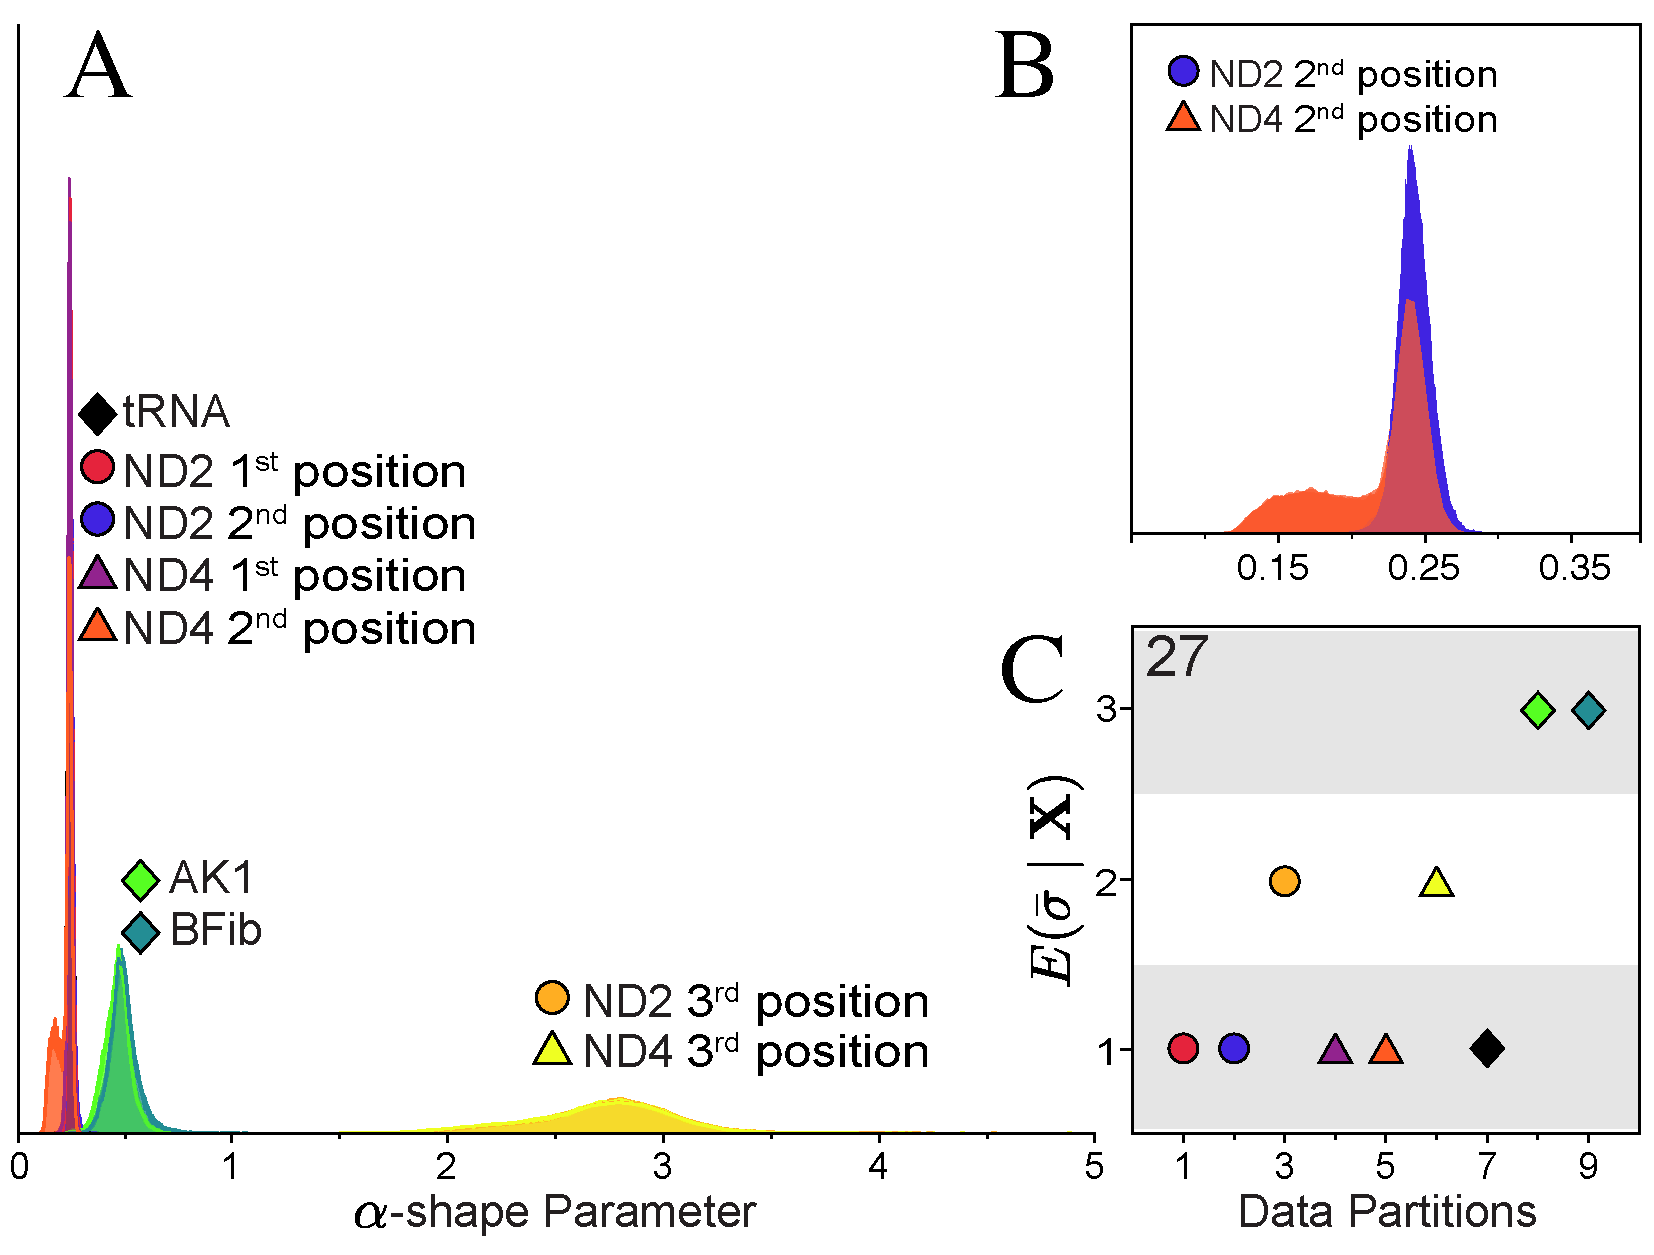
\includegraphics[width=120mm]{figures/figure_1} 
\end{figure} 

\newpage

\begin {center} 
{\sc Figure 2}
\end{center}

\vspace{1.0in}

\begin{figure}[h] 
\centering 
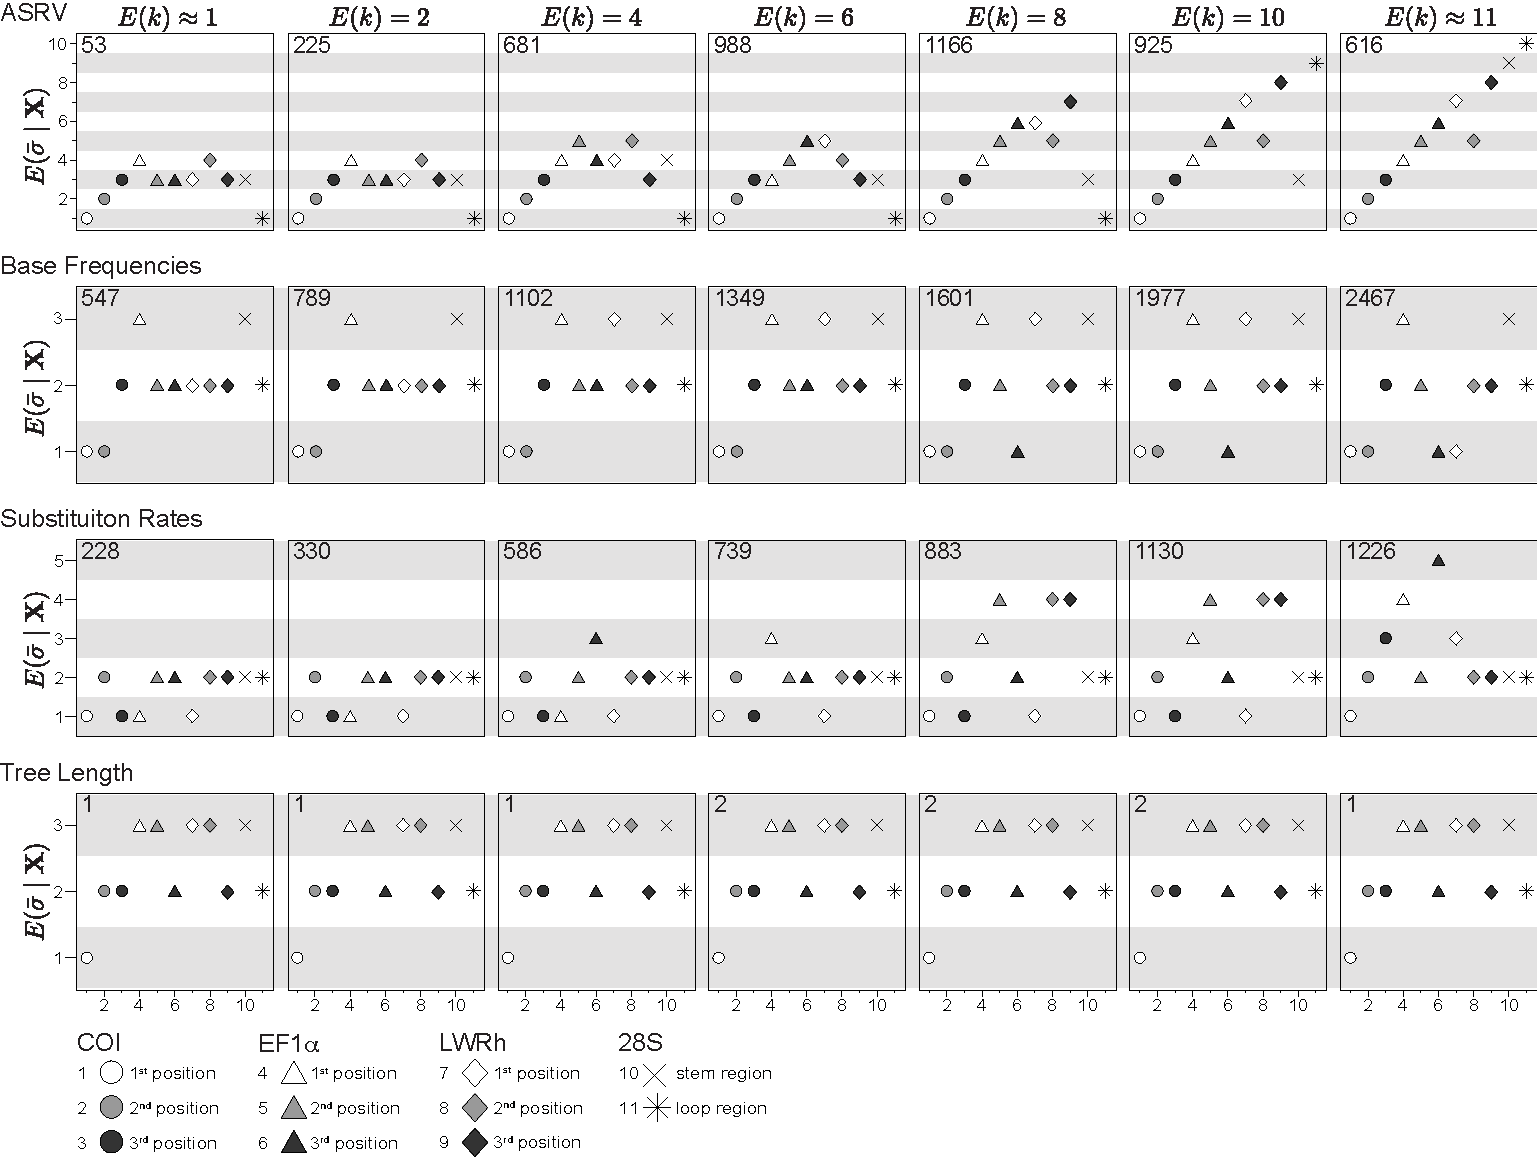
\includegraphics[angle=90, height=175mm]{figures/figure_2} 
\end{figure} 

\newpage

\begin {center} 
{\sc Figure 3}
\end{center}

\vspace{1.0in}

\begin{figure}[h] 
\centering 
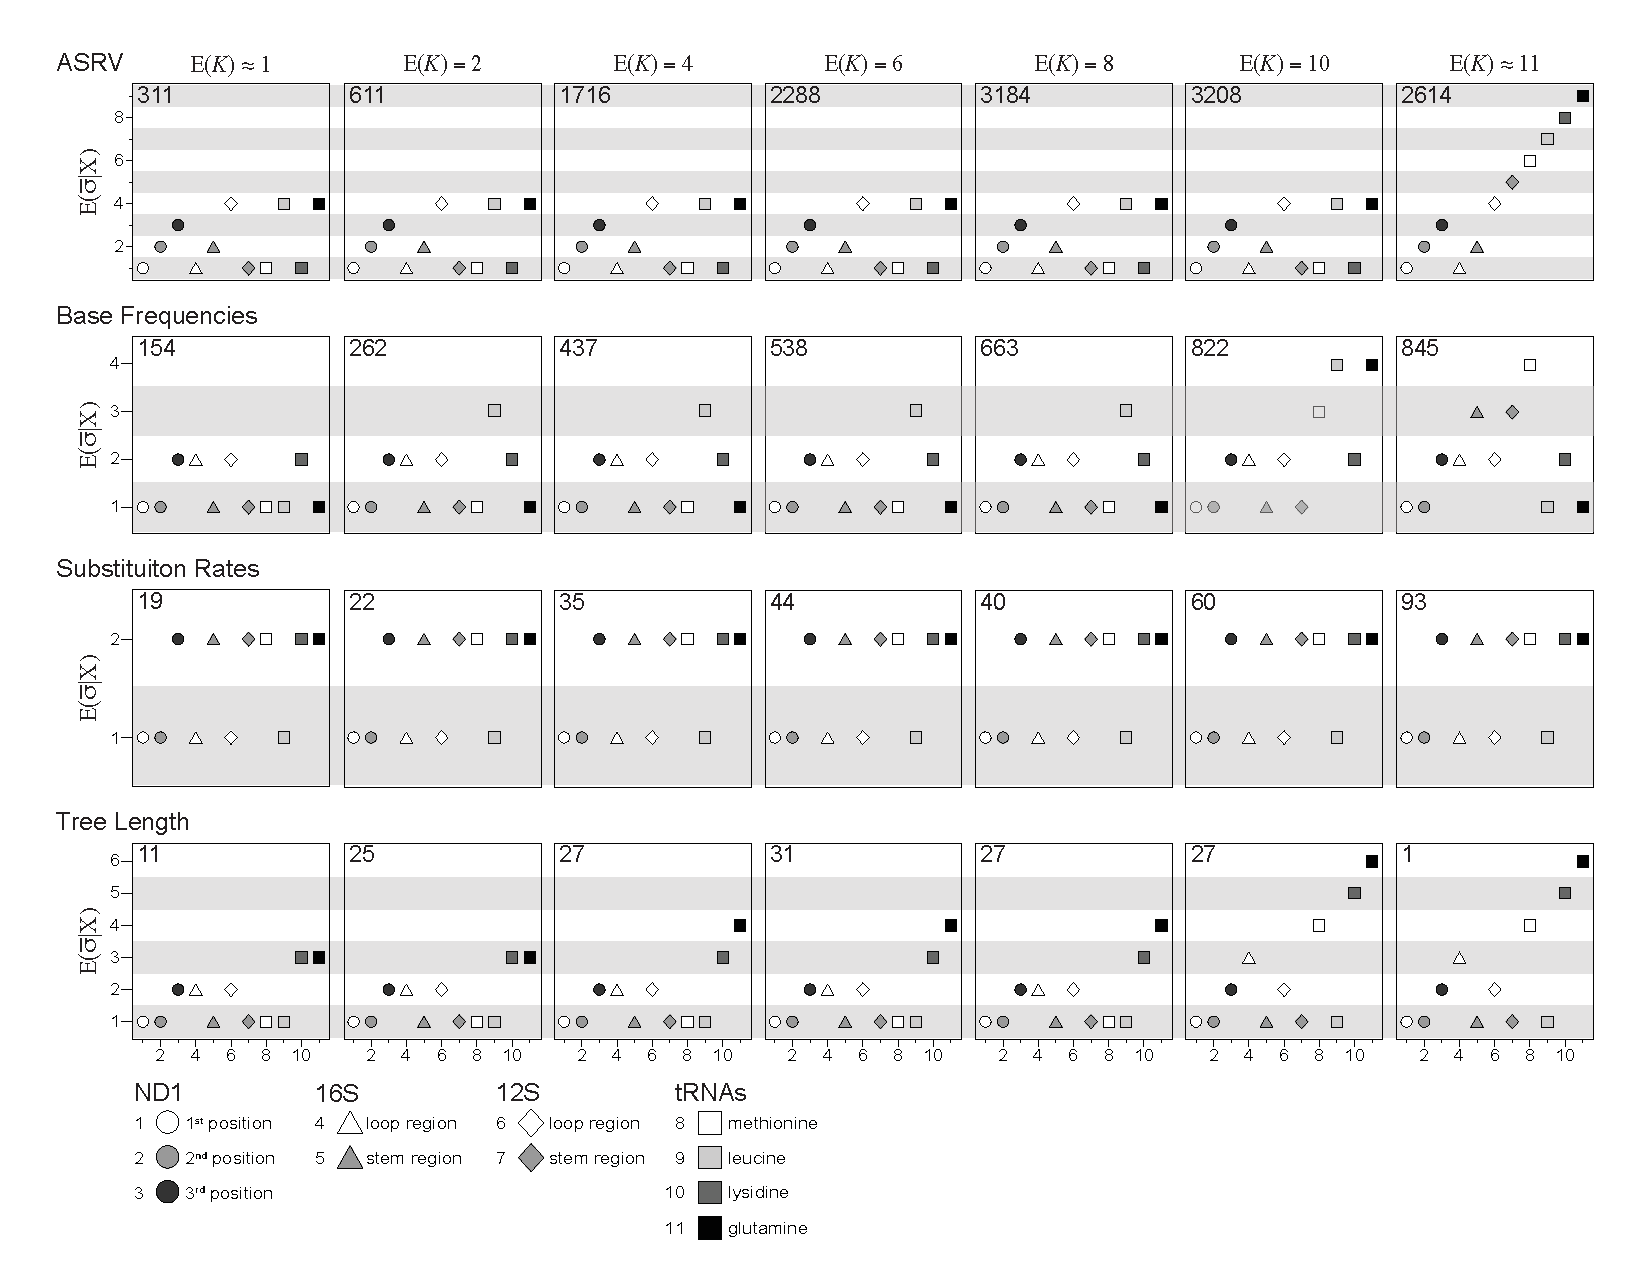
\includegraphics[angle=90, height=175mm]{figures/figure_3} 
\end{figure} 

\newpage

\begin {center} 
{\sc Figure 4}
\end{center}

\vspace{1.0in}

\begin{figure}[h] 
\centering 
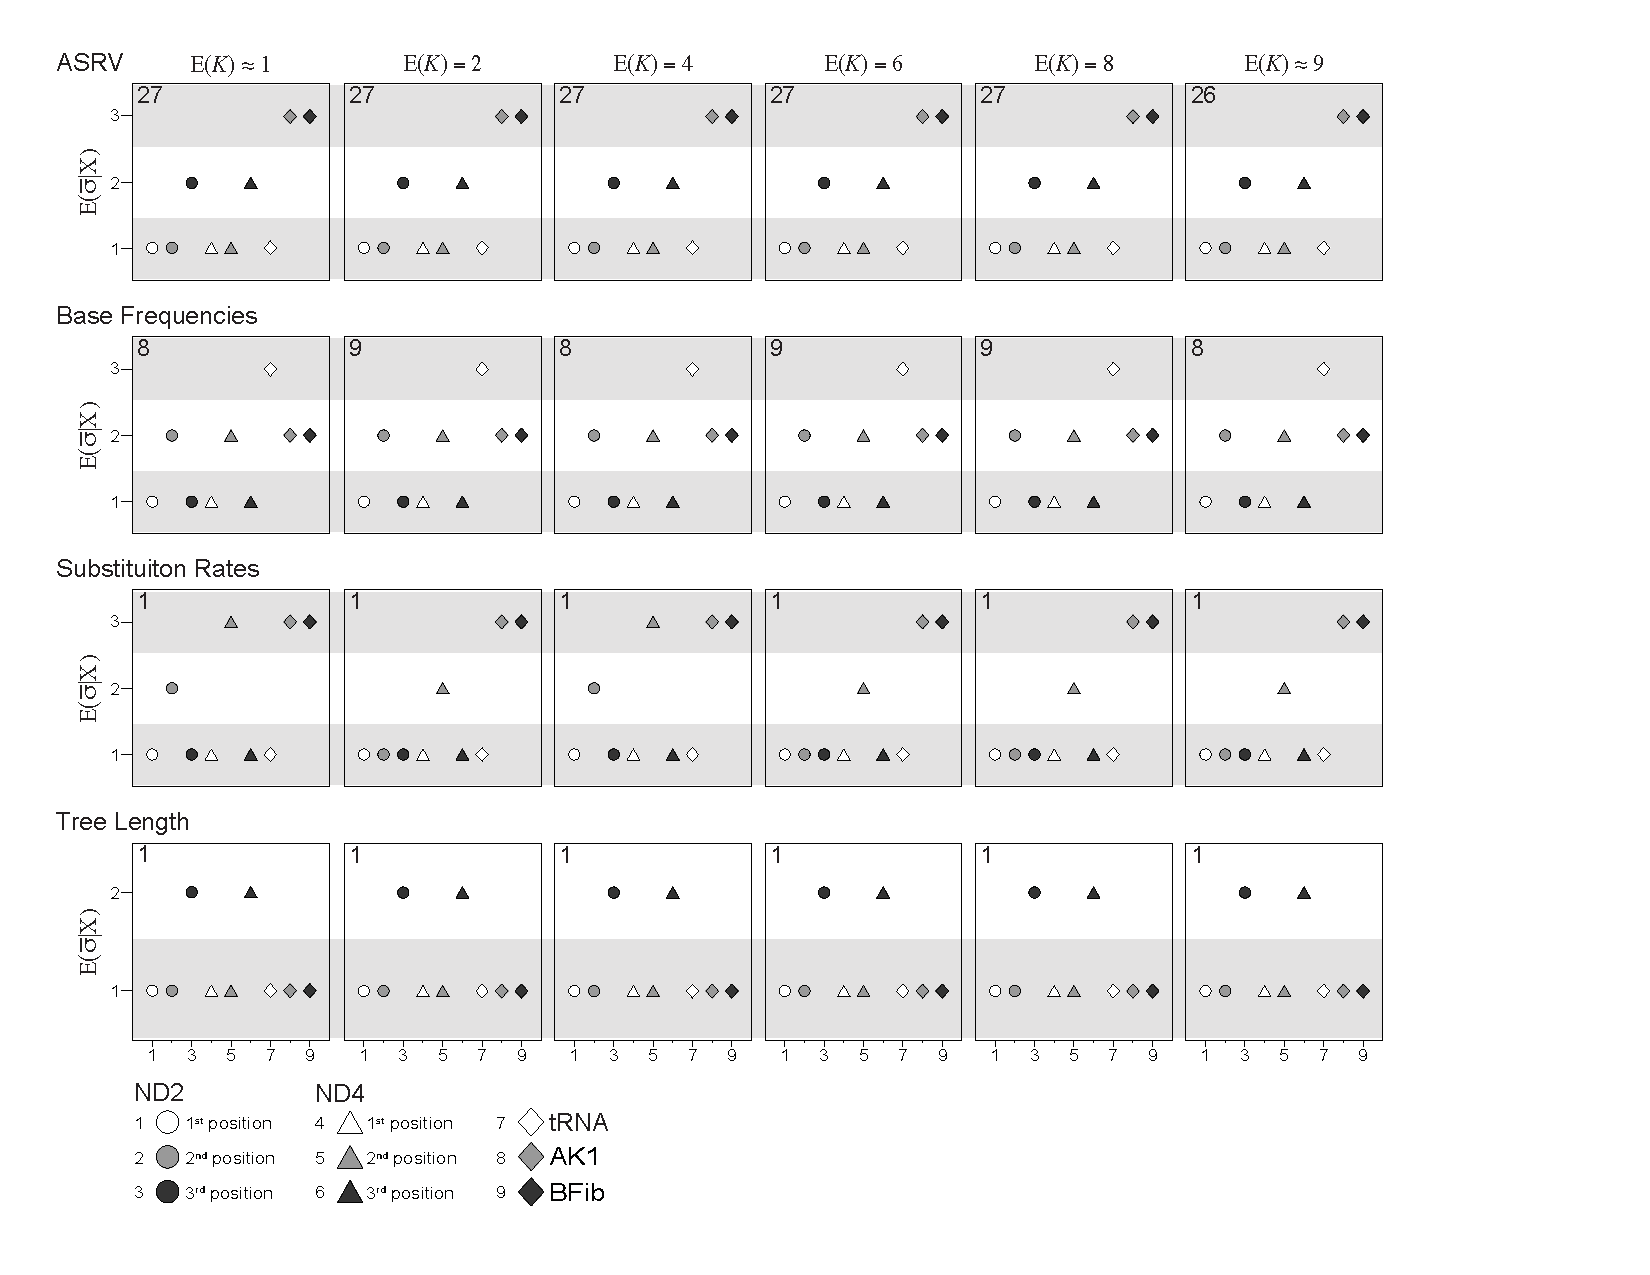
\includegraphics[angle=90, height=175mm]{figures/figure_4} 
\end{figure} 

\newpage

\begin {center} 
{\sc Figure 5}
\end{center}

\vspace{1.0in}

\begin{figure}[h] 
\centering 
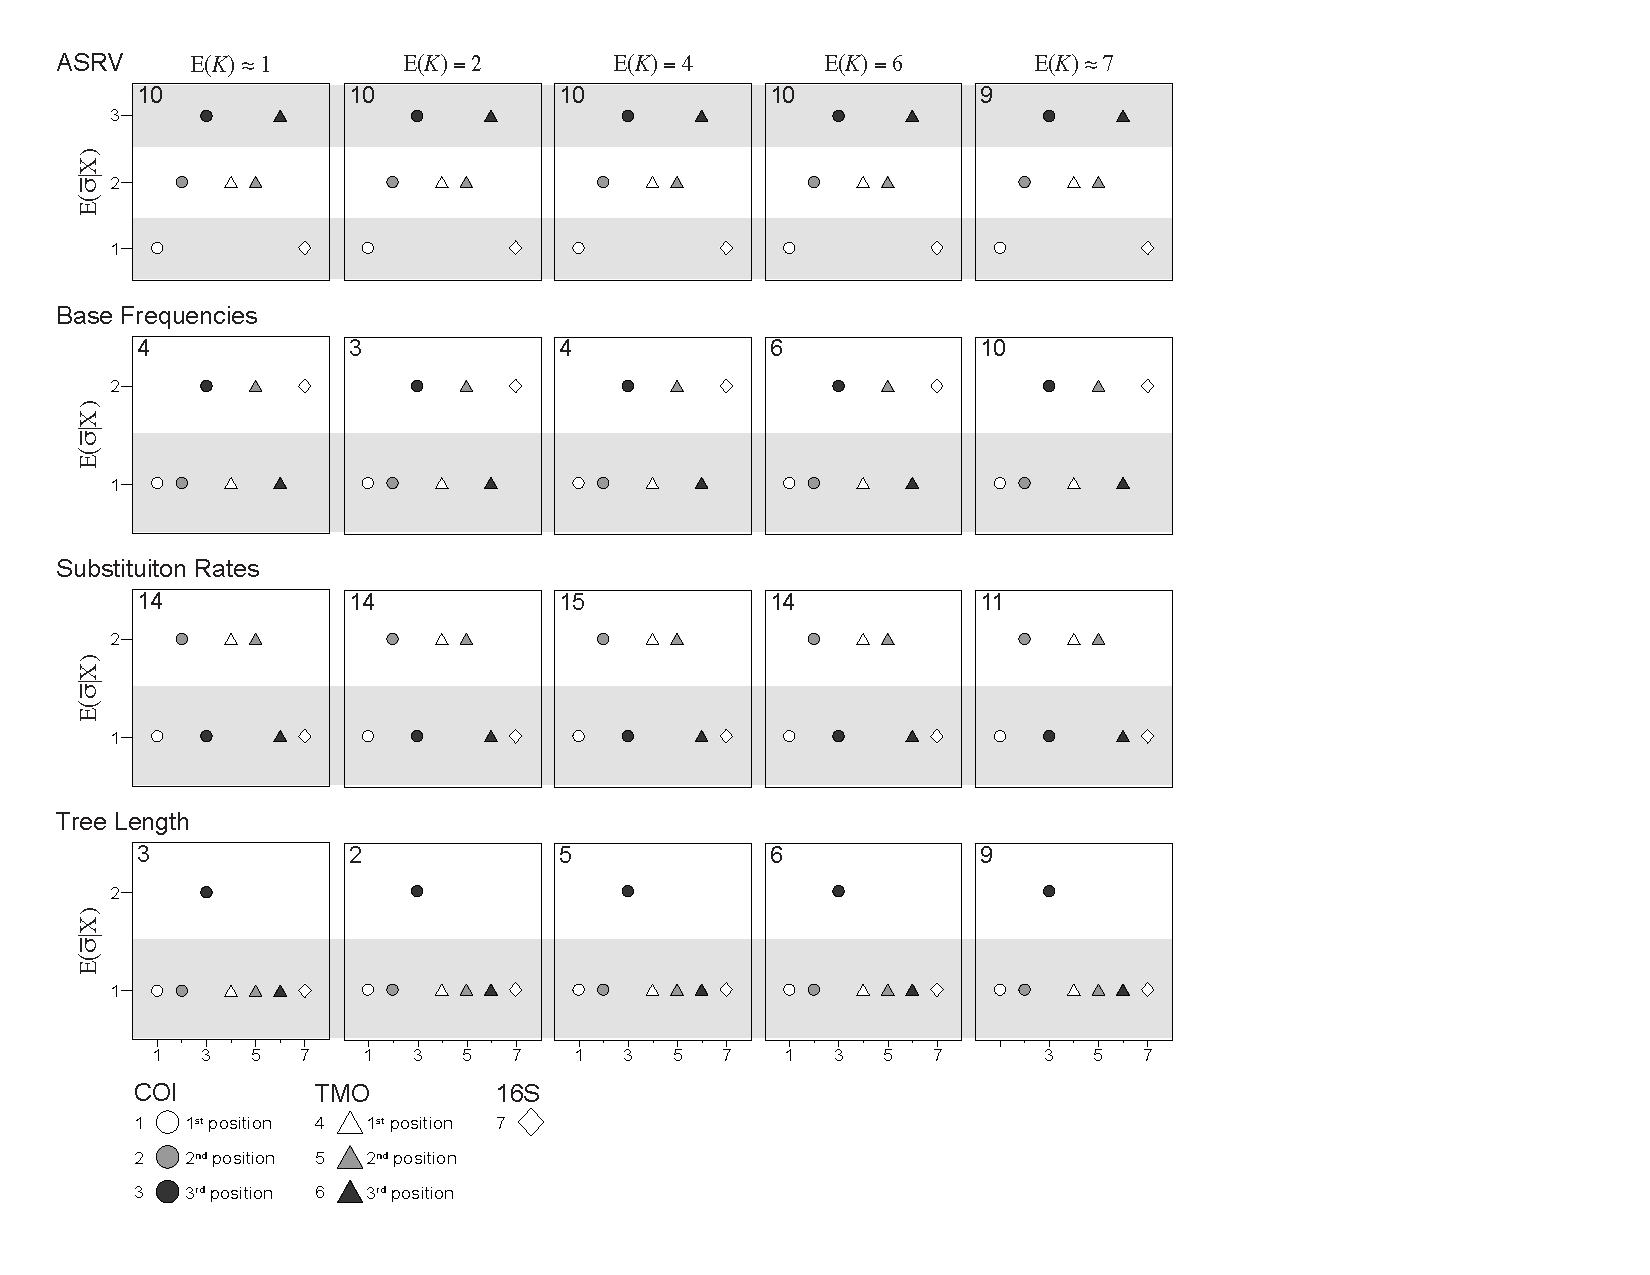
\includegraphics[height=175mm]{figures/figure_5} 
\end{figure} 

\newpage

\begin {center} 
{\sc Figure 6}
\end{center}

\vspace{1.0in}

\begin{figure}[h] 
\centering 
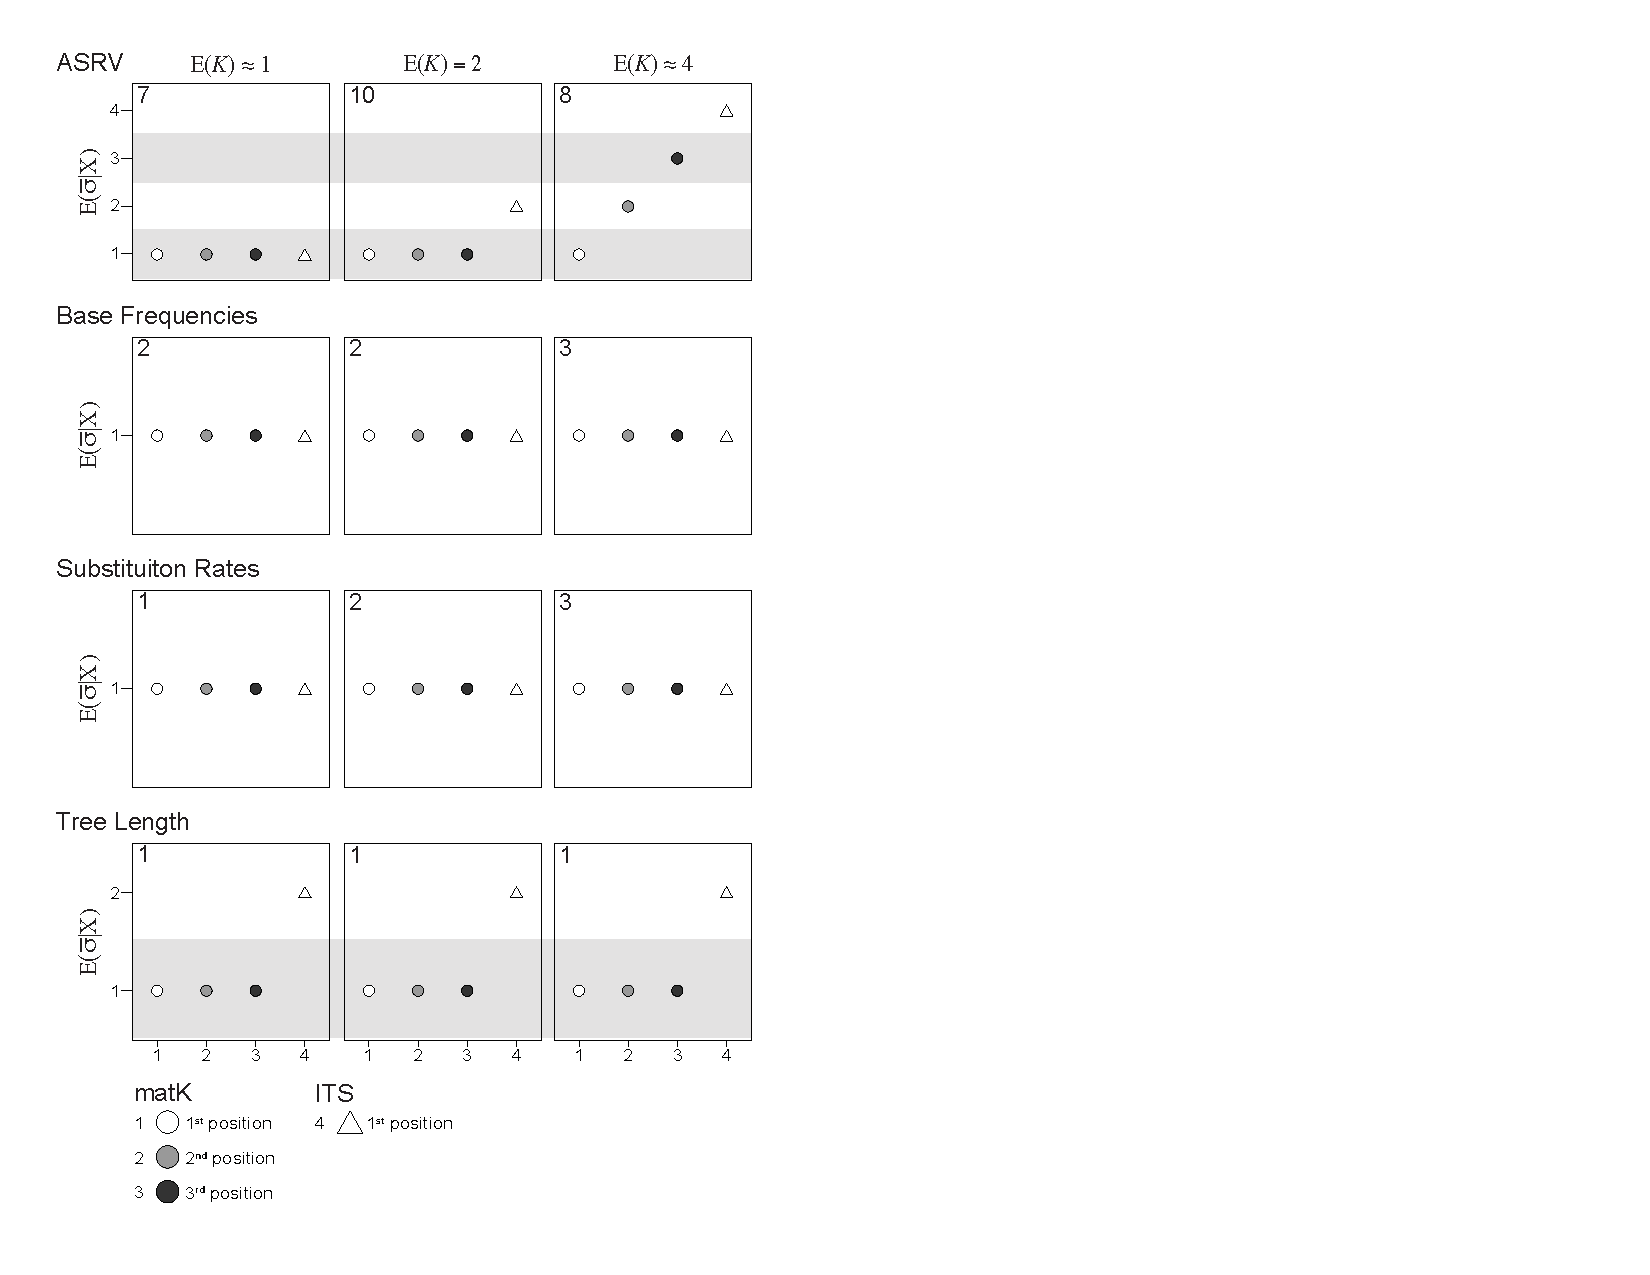
\includegraphics[height=175mm]{figures/figure_6} 
\end{figure} 




\end{document}


 

